\documentclass[UTF8,12pt]{article}

\usepackage[utf8]{inputenc}
\usepackage{ctex}
\usepackage{amsmath,amsfonts,amssymb}
\usepackage{graphicx,epsfig,subfig}
\usepackage{makeidx,hyperref}
\usepackage{geometry}
\usepackage{listings}
\usepackage[linesnumbered,boxed]{algorithm2e}
\usepackage{xcolor}

\geometry{scale=0.8}

%\setlength{\lineskip}{\baselineskip}
\setlength{\parskip}{0.5\baselineskip}

\title{Anderson局部化实验报告2}
\author{flag}
\date{\today}

\begin{document}
    
\maketitle

\section{探究参数何时最优}

\subsection{$\alpha$的选取}

我们先从一维的简单情况开始。一维区间分成20段,K=1000,V是均匀分布的随机数,Neumann边界条件。选取$x_0$为0.5 对不同的$\alpha$模拟。如图\ref{fig1}

\begin{figure}[htbp]
    \centering
    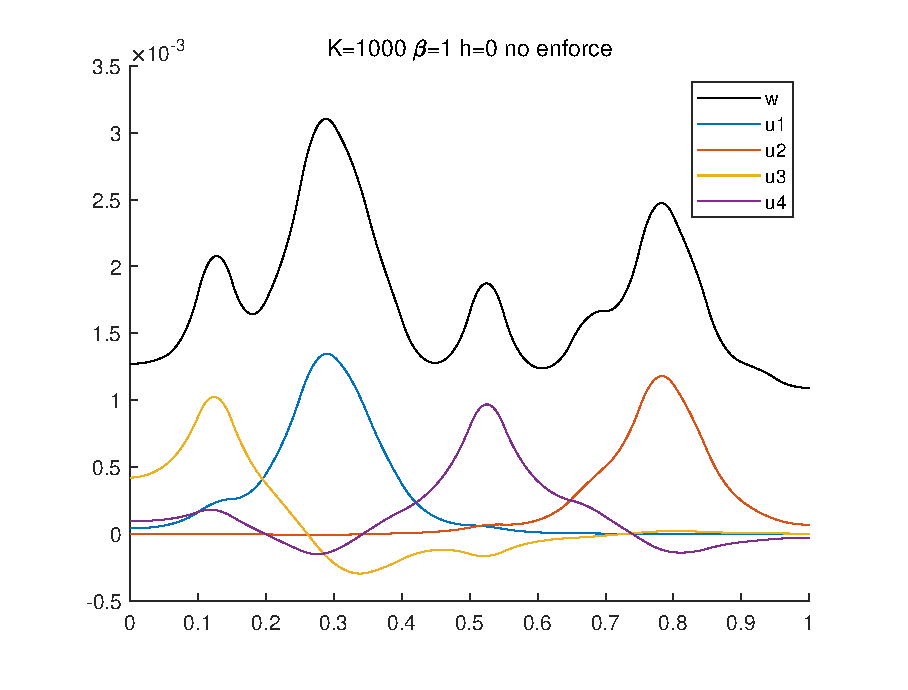
\includegraphics[width=0.3\linewidth]{pic/ua0}
    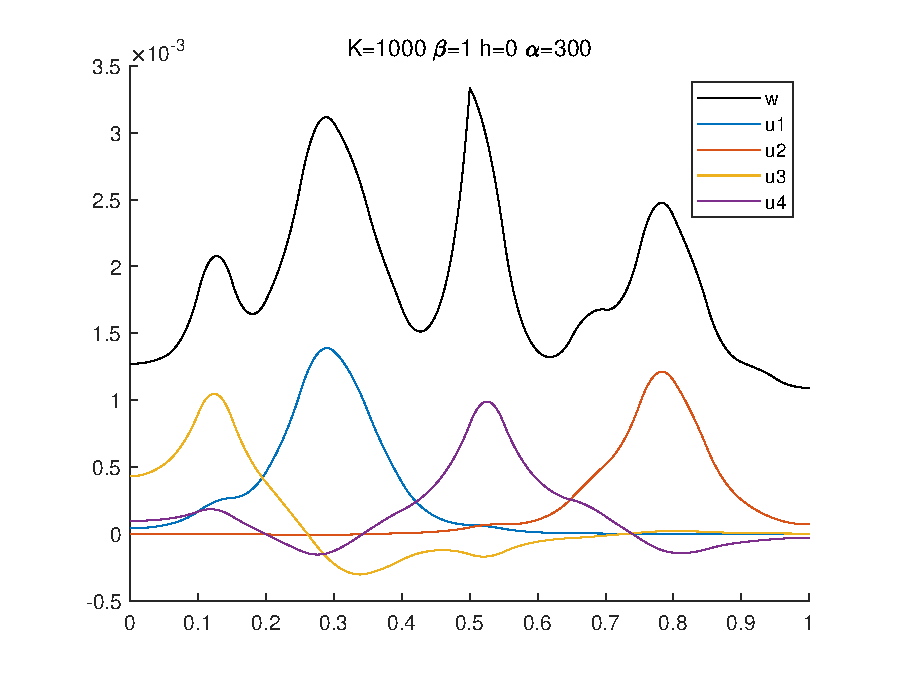
\includegraphics[width=0.3\linewidth]{pic/ua300} \\
    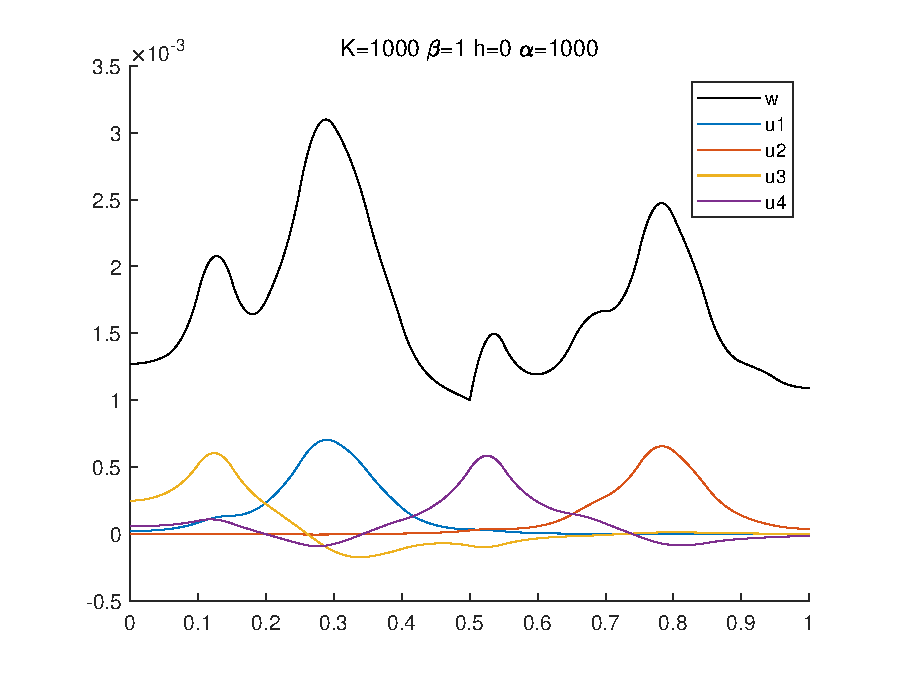
\includegraphics[width=0.3\linewidth]{pic/ua1000}
    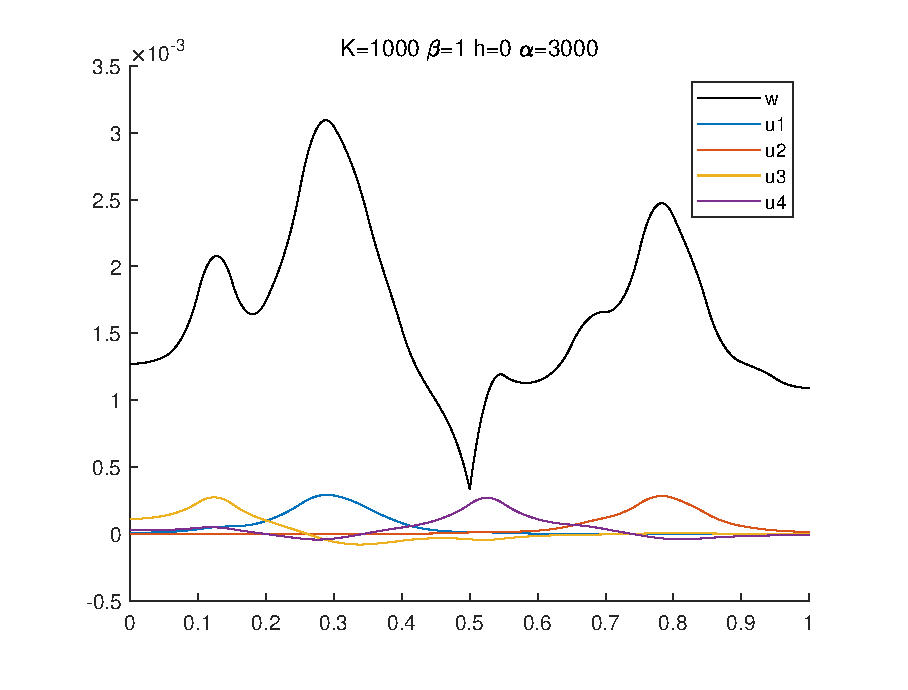
\includegraphics[width=0.3\linewidth]{pic/ua3000}
    \label{fig1}
\caption{一维,不同alpha下的表现}
\end{figure}

可以看到,在$x_0$附近landscape会间断。我们希望的情况是下面彩色的线和上面黑色的线比较靠近。可以看出,没有enforce的landscape是四幅图里最优的。

把四条landscape画在一起,发现强制的边界仅仅改变了$x_0$附近的函数值,对更远的地方就没有效果了。在二维情况,这种现象特别特别明显。如图\ref{fig2}。图中二维分割成$20 \times 20$的小块,$\alpha = 200$其他参数同上。

\begin{figure}[htbp]
    \centering
    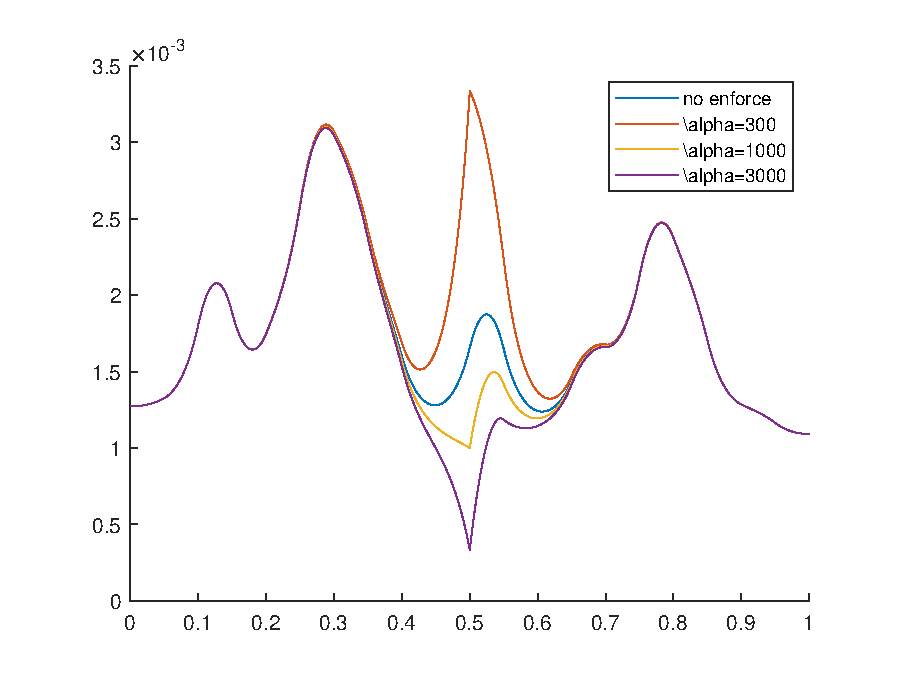
\includegraphics[width=0.3\linewidth]{pic/nouse1d}
    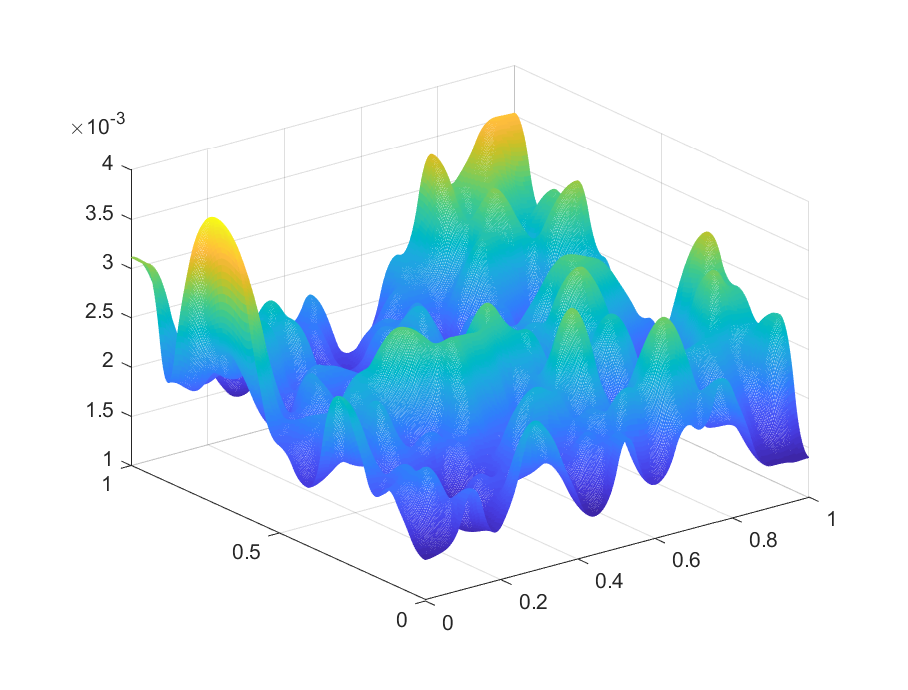
\includegraphics[width=0.3\linewidth]{pic/nouse2d1}
    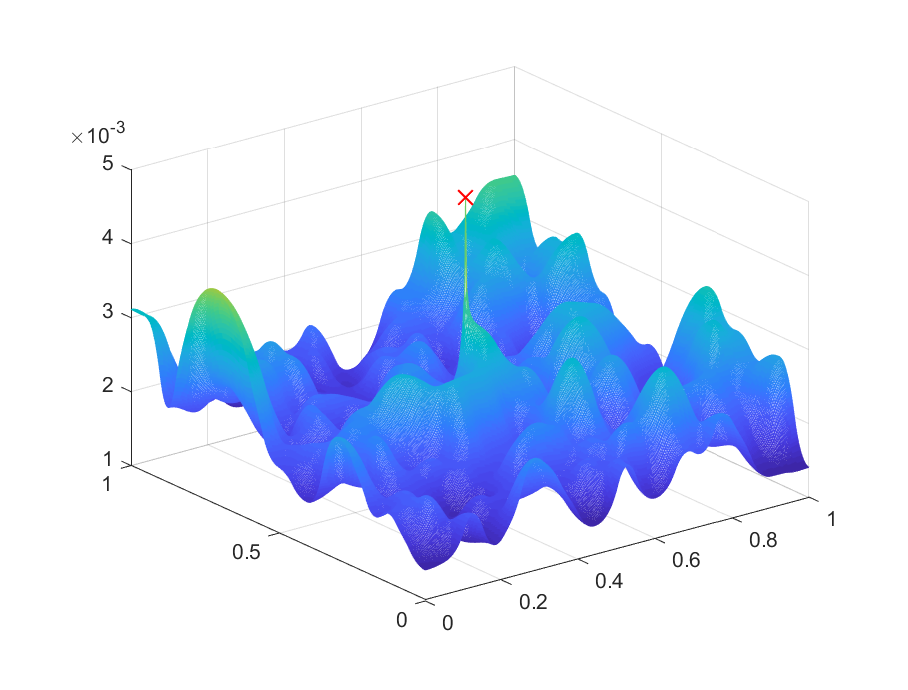
\includegraphics[width=0.3\linewidth]{pic/nouse2d2}
    \label{fig2}
\caption{左图是一维的情况,中间是no enforce的二维曲面,右边是把(0.5, 0.5)处强行设成1/200的曲面。红叉下面那个特别细的就是enforce对它的影响。}
\end{figure}

综合以上现象,我觉得$\alpha$直接选成landscape最大值的倒数就好。

\subsection{$\beta$的选取}

首先在一维情况下实验,Robin边界条件,取h=1,其他参数同上。结果如图\ref{fig3}
\begin{figure}[htbp]
    \centering
    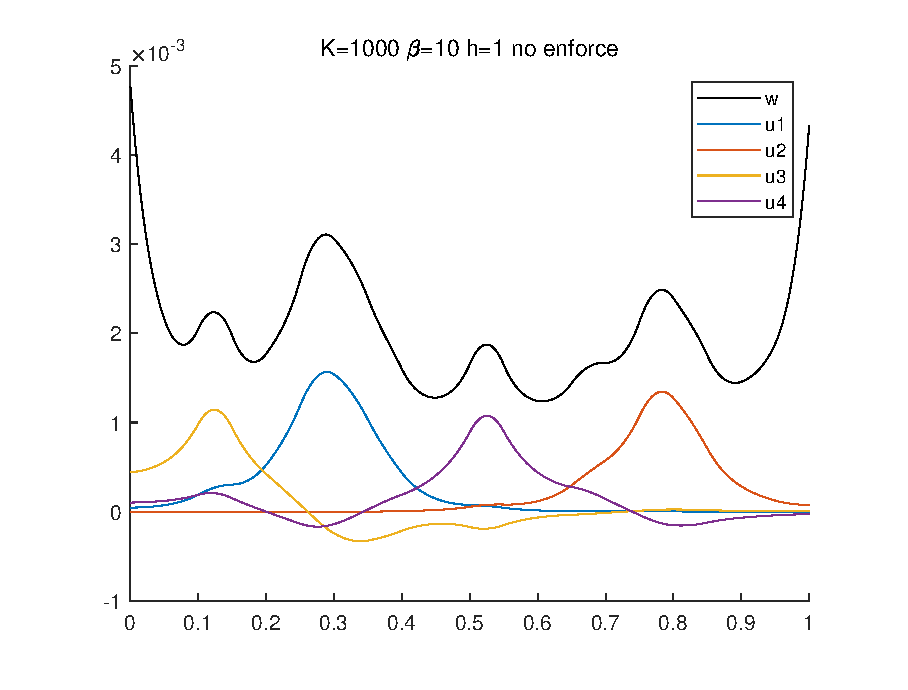
\includegraphics[width=0.3\linewidth]{pic/h1b10}
    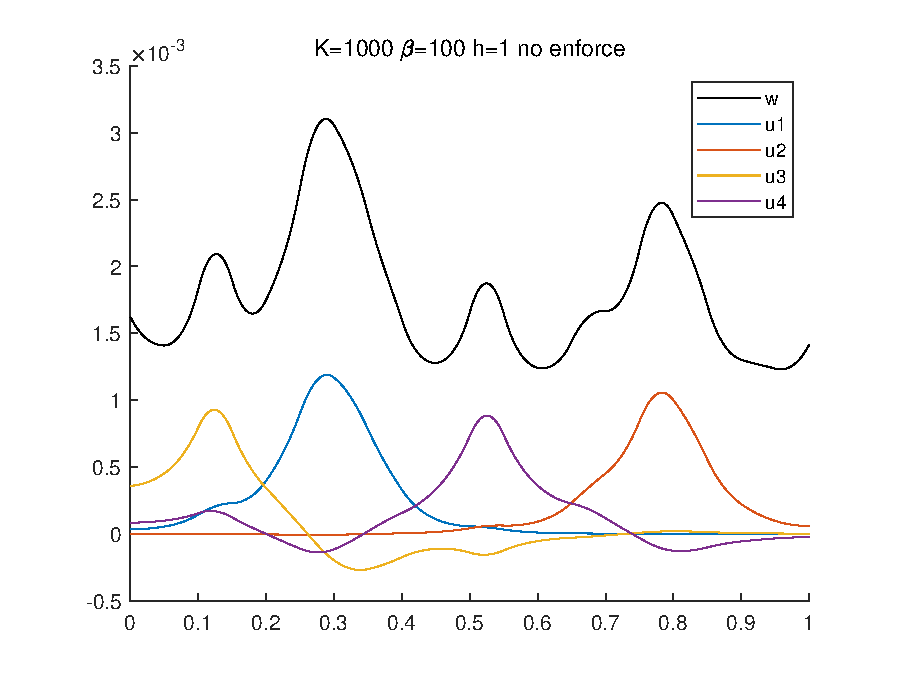
\includegraphics[width=0.3\linewidth]{pic/h1b100}
    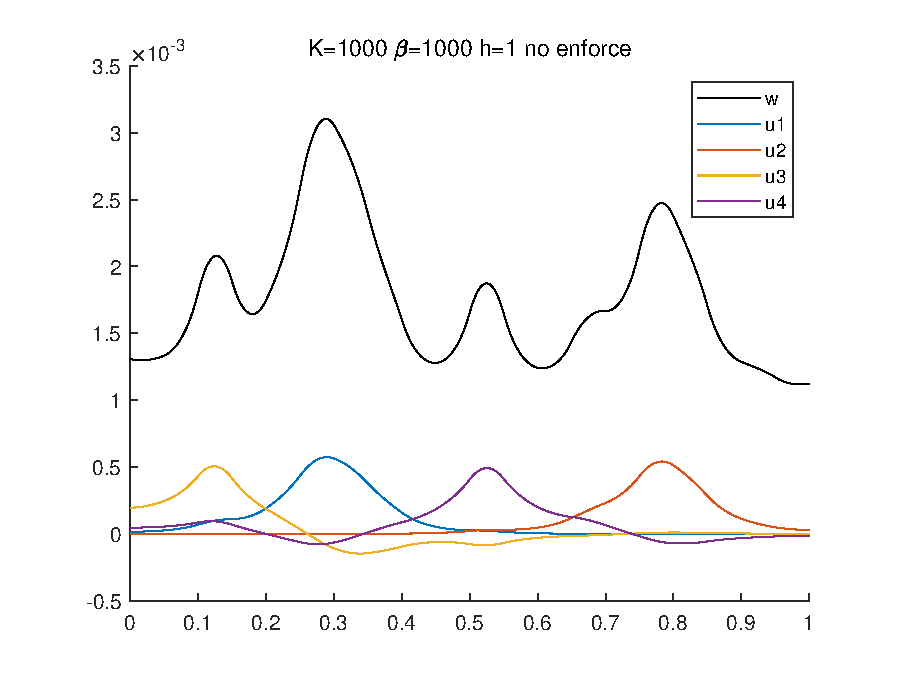
\includegraphics[width=0.3\linewidth]{pic/h1b1000}
    \label{fig3}
\caption{beta对结果的影响}
\end{figure}

从图中可以看出,$\beta$不能太小,否则边界会翘起来,也不能太大,否则不等式就不精确了。之前猜测$\beta$应该大概取成$Kh$,现在看起来并不是这样。

同样,$\beta$的选取仅仅影响landscape在边界附近的性质,对内部影响比较小。如图\ref{fig4}

\begin{figure}[htbp]
    \centering
    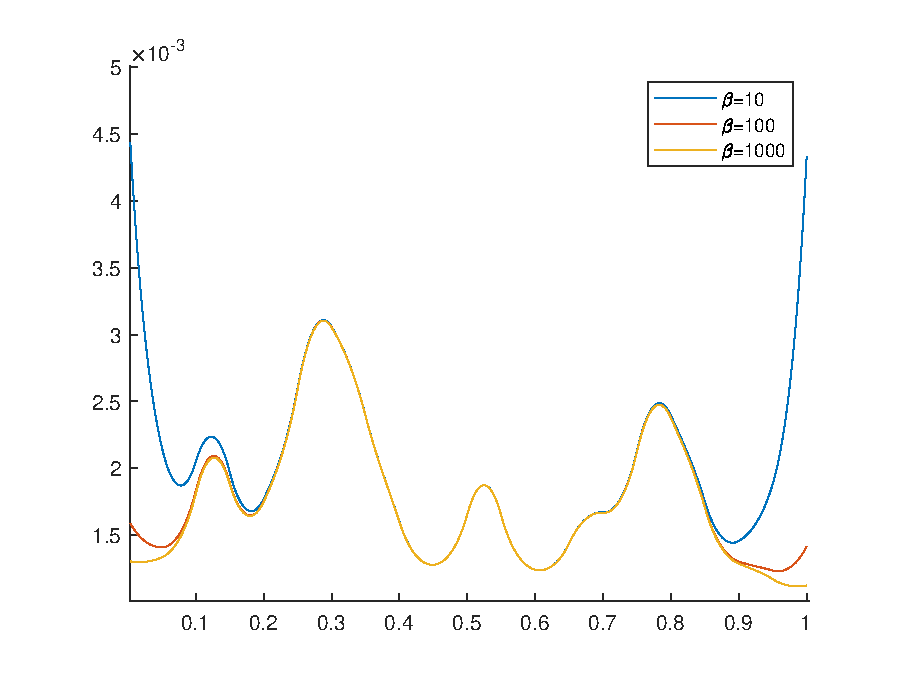
\includegraphics[width=0.4\linewidth]{pic/nouseb1d}
    \label{fig4}
\caption{beta对结果的影响}
\end{figure}

对于什么样的参数是“最优”,并没有一个确切的有指标刻画的标准。对于$\beta$具体取什么样的值比较好,现在只能说可以在边界不会翘起来的情况下,可以尽量取得小一点。

\subsection{localize到边界时参数的选取}

之前有一个问题是当localize的位置在边界时,要如何选取$\beta$的值,这时的结果会不会有变化。我们用同样的势函数,换不同的$\beta$模拟。结果如图\ref{fig9}。得到的结果和原来差不多。由于在最终的不等式里出现的是$\beta$和特征值相加,所以$\beta$选取和特征值在同一数量级的数就差不多。

\begin{figure}[htbp]
    \centering
    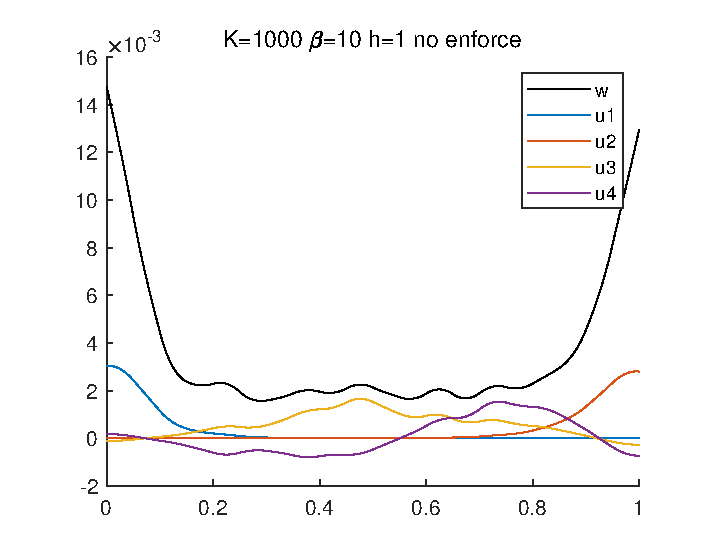
\includegraphics[width=0.3\linewidth]{pic/bdb2}
    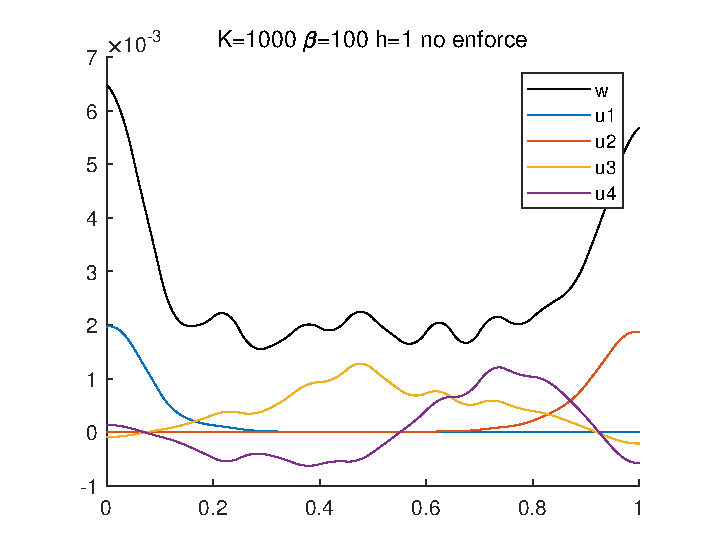
\includegraphics[width=0.3\linewidth]{pic/bdb3}
    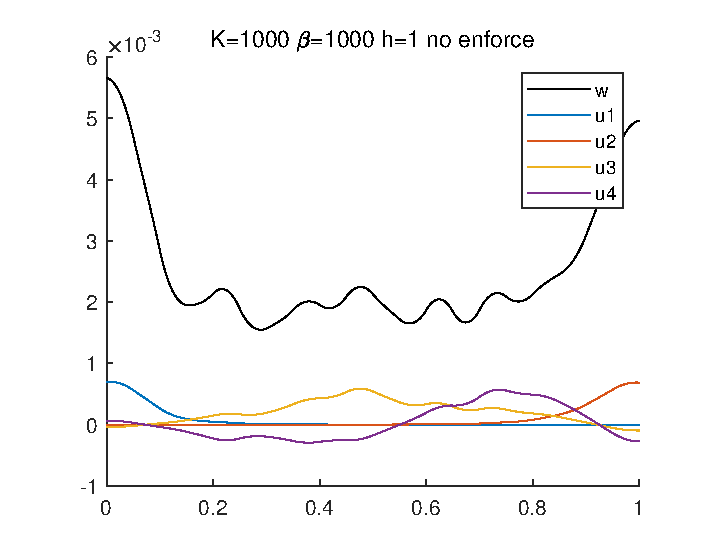
\includegraphics[width=0.3\linewidth]{pic/bdb4}
    \label{fig9}
\caption{localize到边界的landscape}
\end{figure}

\section{不同边界条件下的比较}

在实验中我们发现,边界条件是Dirichlet还是导数型的,主要影响landscape的边界,对landscape的内部影响较小。对eigenmode的影响就比较大,因为原来不会聚集到边界的峰有可能聚集到边界了。

还是先看一维的情况,在一个特定的V下模拟,这里的V故意在边界选取得比较小,能够突出局部化到边界的效果。如图\ref{fig6}

\begin{figure}[htbp]
    \centering
    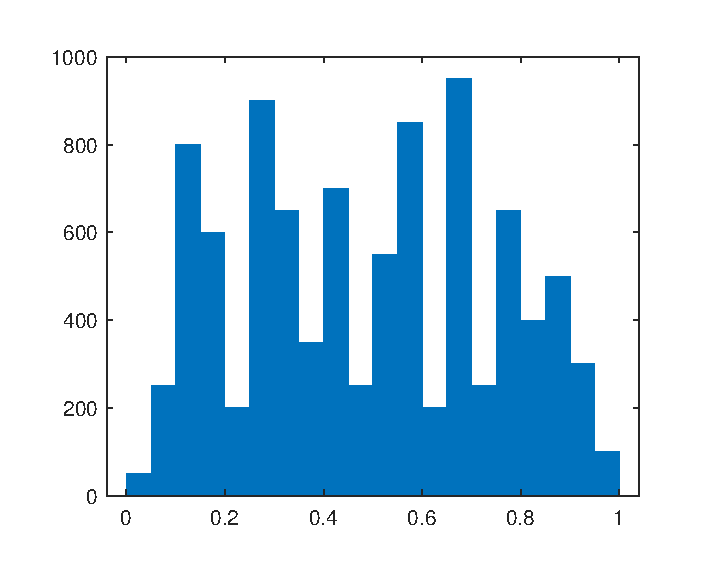
\includegraphics[width=0.3\linewidth]{pic/bdnu1}
    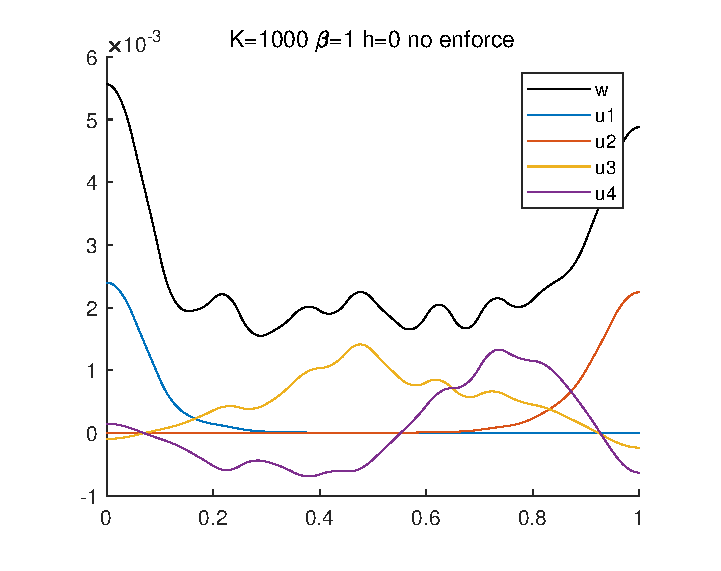
\includegraphics[width=0.3\linewidth]{pic/bdnu2} \\
    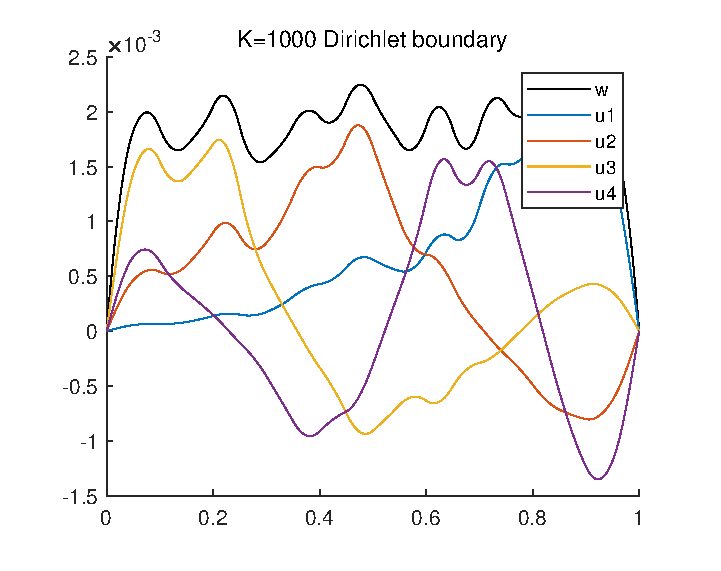
\includegraphics[width=0.3\linewidth]{pic/bdnu3}
    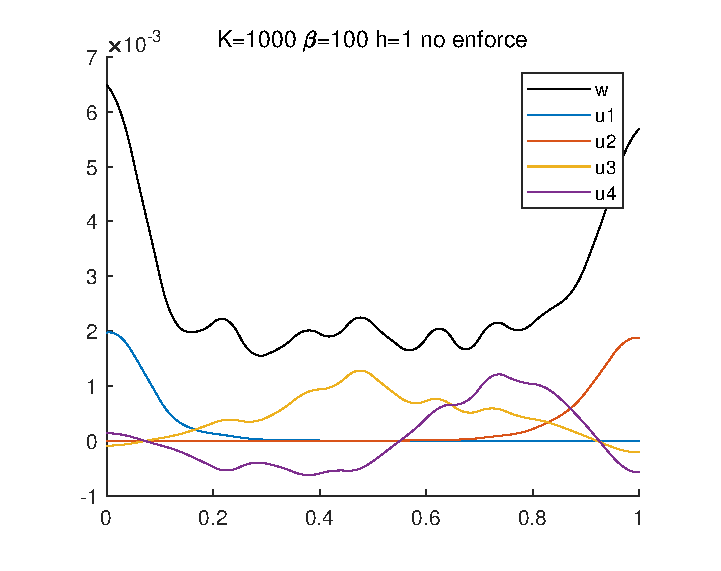
\includegraphics[width=0.3\linewidth]{pic/bdnu4}
    \label{fig6}
\caption{左上为V,剩下三个是不同边界条件下的模拟结果}
\end{figure}

这三个eigenmode很不一样,尤其是Dirichelt和Neumann边界的,相差很多。但是把它们的landscape画在一起,就会发现在内部很相似。图\ref{fig7}中比较了不同边界条件下的landscape。

\begin{figure}[htbp]
    \centering
    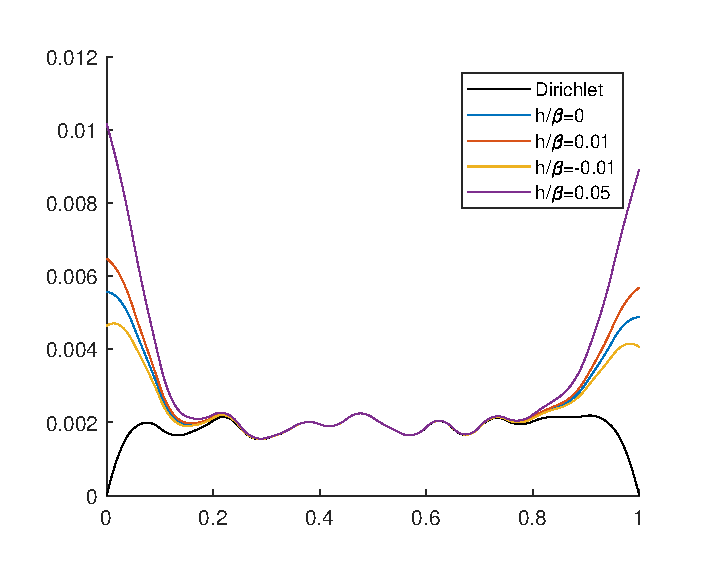
\includegraphics[width=0.4\linewidth]{pic/bdnu5}
    \label{fig7}
\caption{不同边界条件下的landscape}
\end{figure}

二维的也一样。二维的曲面画在一起不容易看清楚,我们只能画切面图。如图\ref{fig8}。landscape在内部差不多。在y=0和y=1的时候就不一样了。

\begin{figure}[htbp]
    \centering
    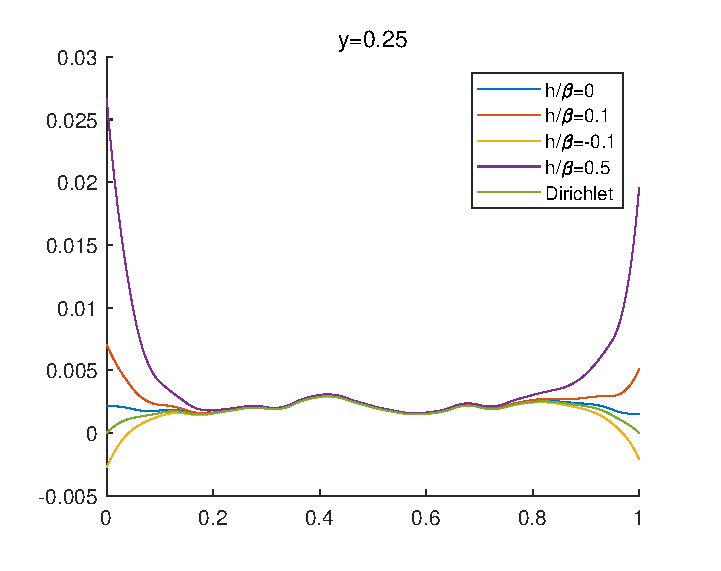
\includegraphics[width=0.3\linewidth]{pic/bdny25}
    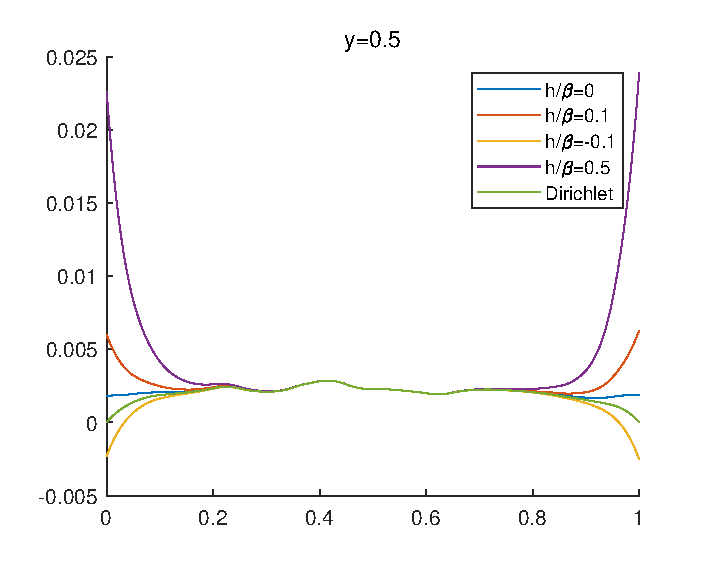
\includegraphics[width=0.3\linewidth]{pic/bdny5}
    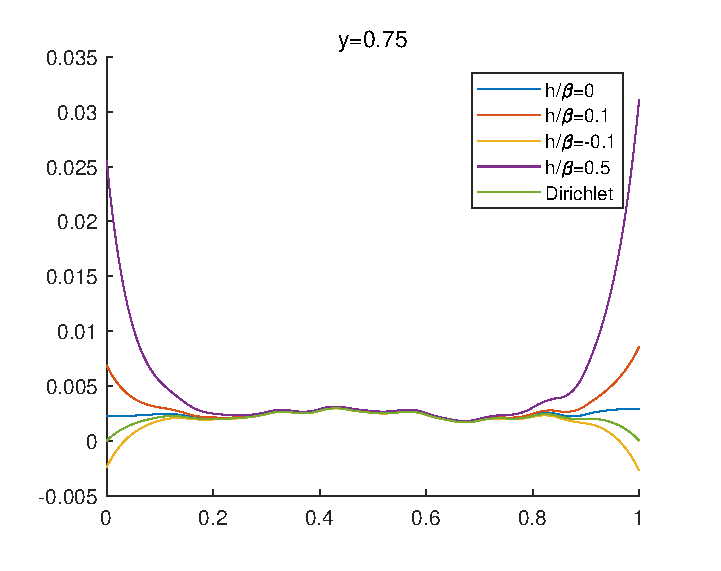
\includegraphics[width=0.3\linewidth]{pic/bdny75}
    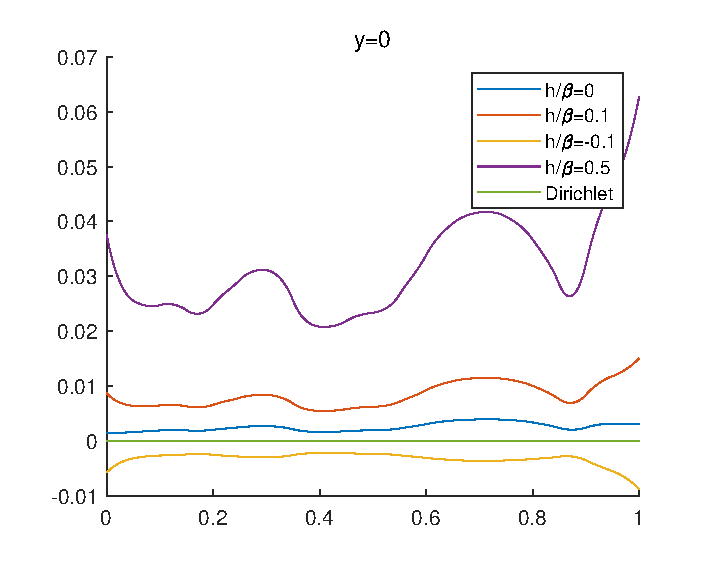
\includegraphics[width=0.3\linewidth]{pic/bdny0}
    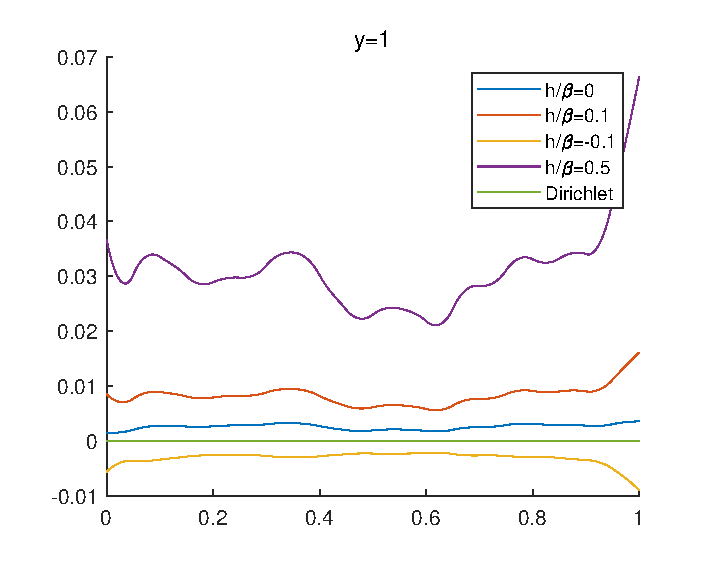
\includegraphics[width=0.3\linewidth]{pic/bdny1}
    \label{fig8}
\caption{二维不同边界条件下的landscape}
\end{figure}

\section{多算几个特征值}

根据测试,现有的代码至少可以计算50个以内的最小特征值,更多的说不定也可以。测试过程中,用50x50的分块,求解了50个特征值,只用了40秒就收敛了。这样的表现应该可以达到要求。

我们希望知道不同边界条件下会不会对较大特征值对应的特征函数产生影响。我们还是先看一维的情况。在图\ref{fig10}中我们比较了不同边界条件下的特征值。

\begin{figure}[htbp]
    \centering
    \includegraphics[width=0.24\linewidth]{pic/mei0}
    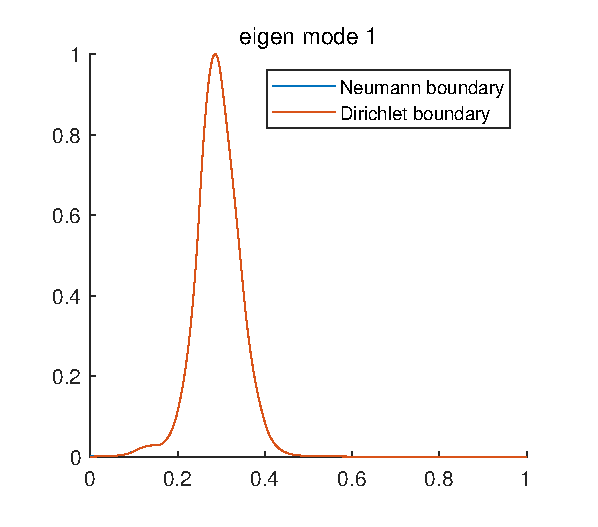
\includegraphics[width=0.24\linewidth]{pic/mei1}
    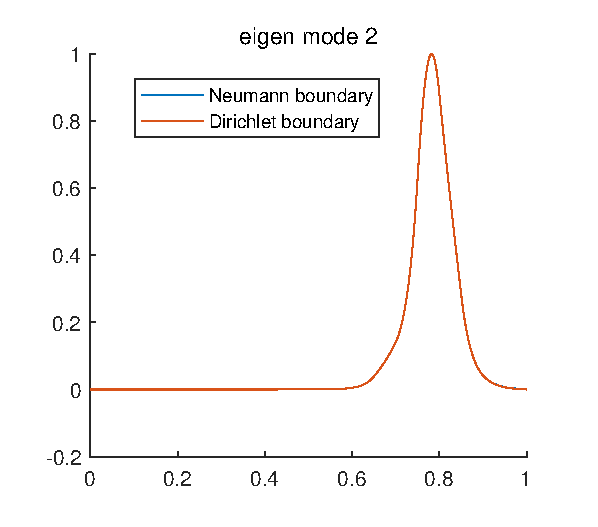
\includegraphics[width=0.24\linewidth]{pic/mei2}
    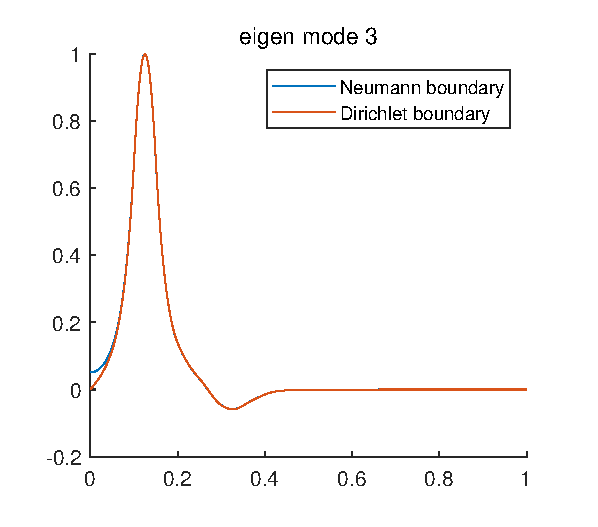
\includegraphics[width=0.24\linewidth]{pic/mei3}
    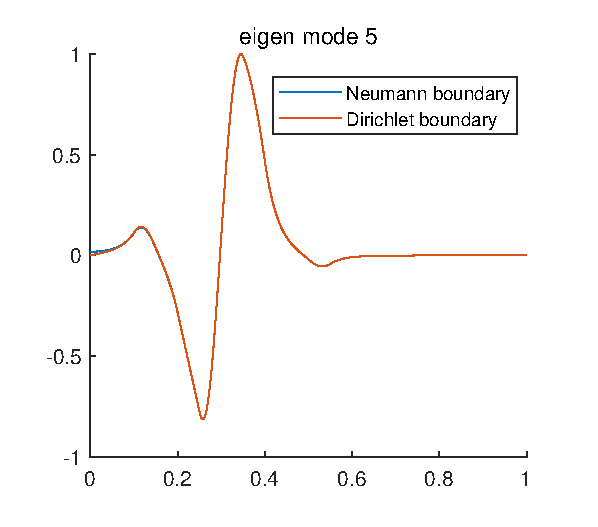
\includegraphics[width=0.24\linewidth]{pic/mei5}
    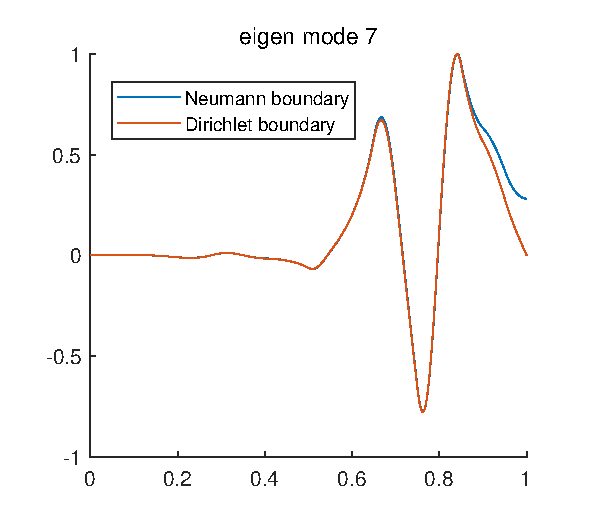
\includegraphics[width=0.24\linewidth]{pic/mei7}
    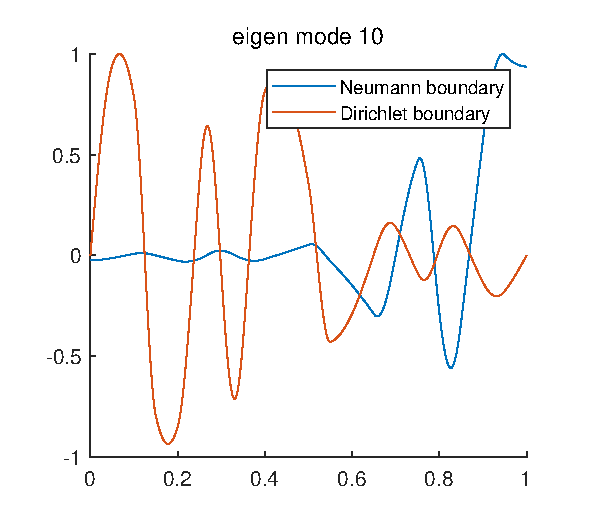
\includegraphics[width=0.24\linewidth]{pic/mei10}
    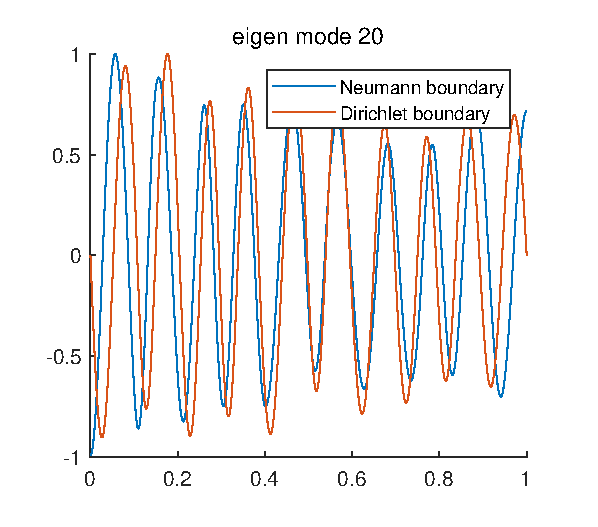
\includegraphics[width=0.24\linewidth]{pic/mei20}
    \label{fig10}
\caption{不同边界条件下eignemode的比较(右上第一张为势函数V)}
\end{figure}

得到的结论和我们的直觉相反,对前几个特征值,两种边界条件下的结果都一样,但是对后面的特征值,两种边界条件下就表现出了很大差异。注意到这个例子中没有前几个特征值localize到边界的情况,我们尝试模拟一下前面提到过的特殊选取,让特征函数出现在边界。如图\ref{fig11}

\begin{figure}[htbp]
    \centering
    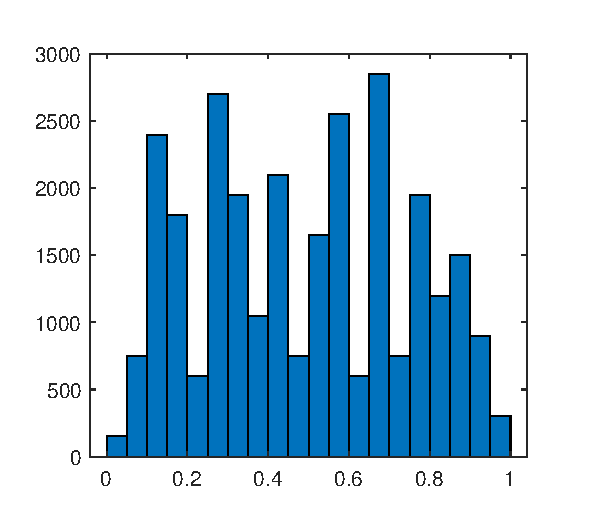
\includegraphics[width=0.24\linewidth]{pic/meb0}
    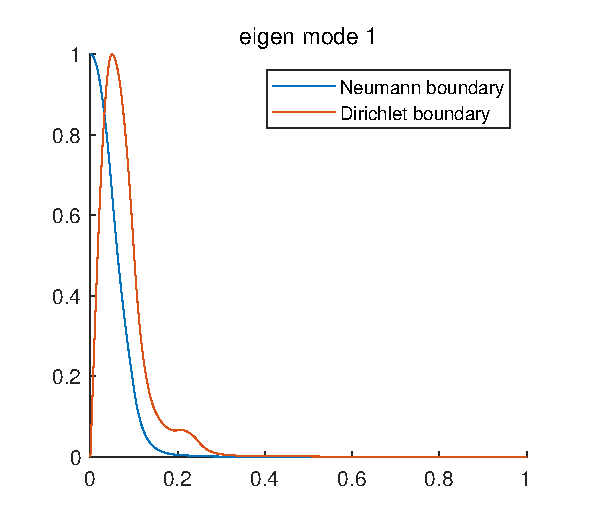
\includegraphics[width=0.24\linewidth]{pic/meb1}
    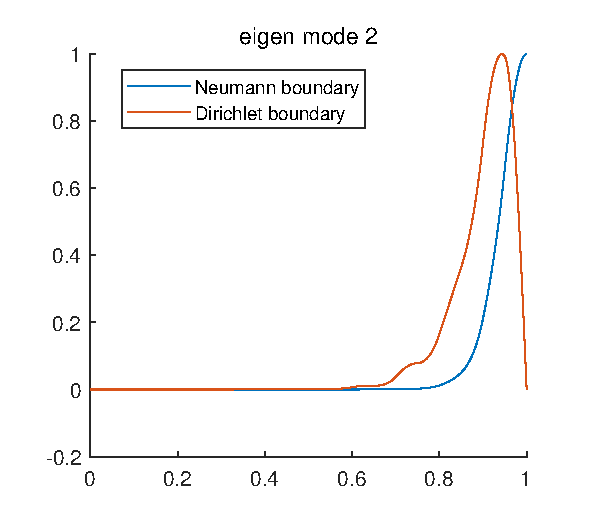
\includegraphics[width=0.24\linewidth]{pic/meb2}
    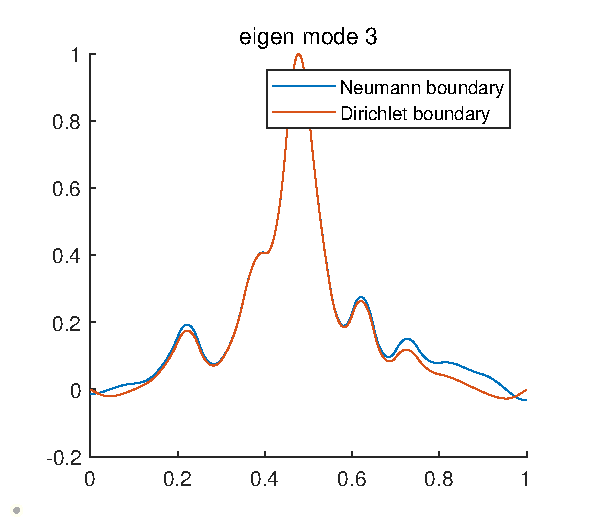
\includegraphics[width=0.24\linewidth]{pic/meb3}
    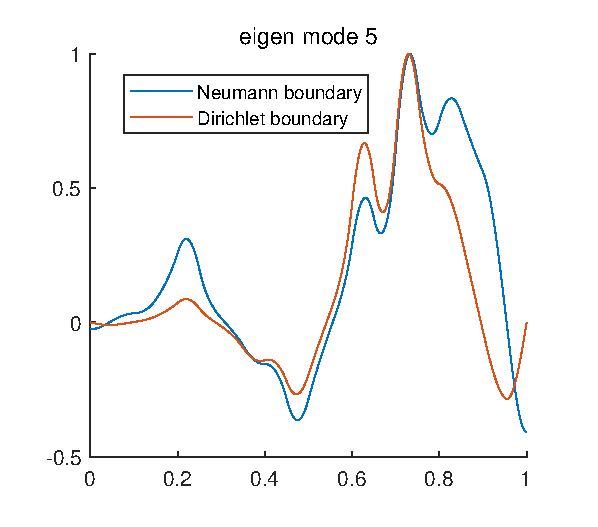
\includegraphics[width=0.24\linewidth]{pic/meb5}
    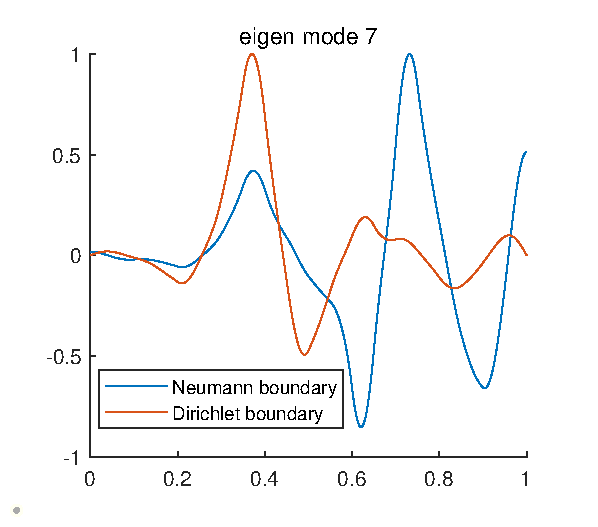
\includegraphics[width=0.24\linewidth]{pic/meb7}
    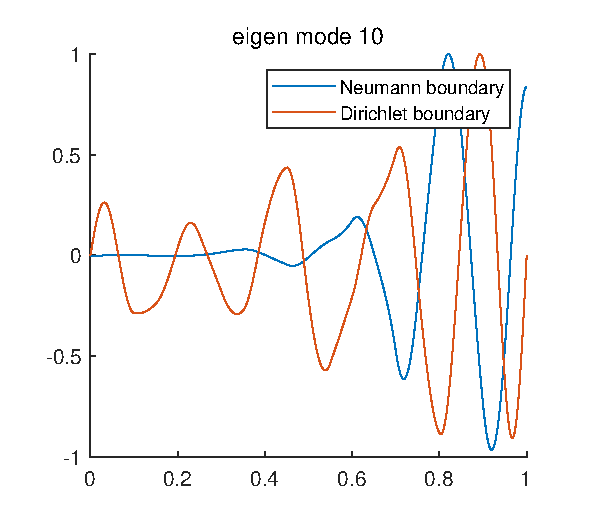
\includegraphics[width=0.24\linewidth]{pic/meb10}
    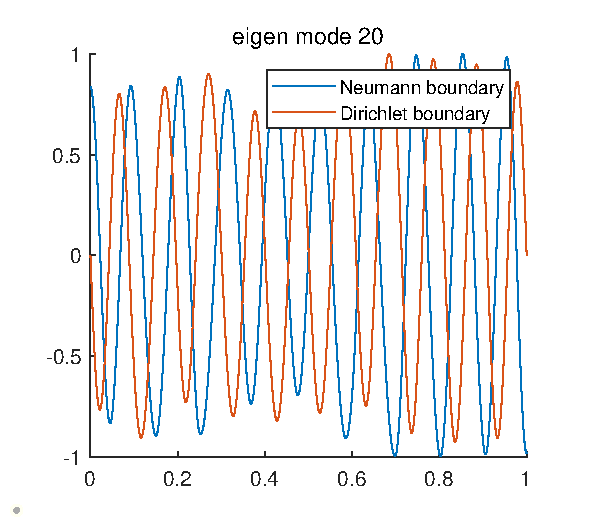
\includegraphics[width=0.24\linewidth]{pic/meb20}
    \label{fig11}
\caption{不同边界条件下eignemode的比较(右上第一张为势函数V)}
\end{figure}

可以看到,除了eigenmode3,其它的都有很大差异。所以我们的结论还是和前面提到的一样:边界条件只影响边界。所以localize到内部的eigenmode不会有影响,如果eigenmode在边界附近出现了峰,那不同的边界条件就会对它影响很大。

下面我们研究二维的情况,如图\ref{fig12}。由于二维的情况大多数都localize在边界,所以两种边界条件下的情况完全不一样。
\begin{figure}[htbp]
    \centering
    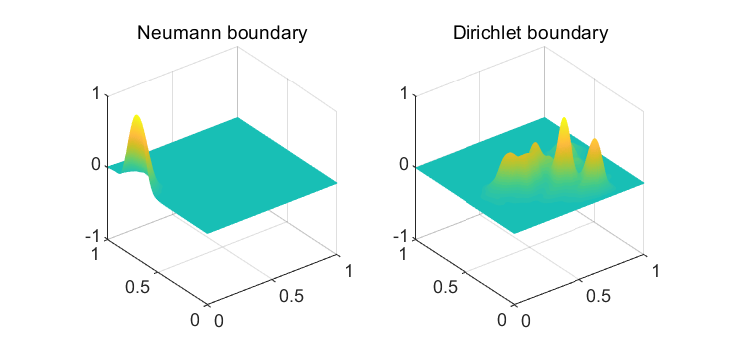
\includegraphics[width=0.45\linewidth]{pic/me2d1}
    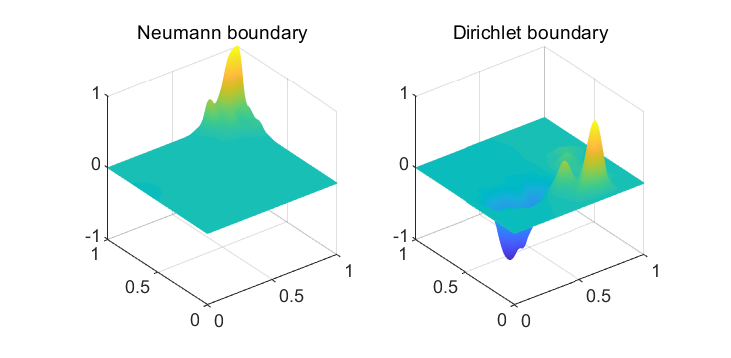
\includegraphics[width=0.45\linewidth]{pic/me2d2}
    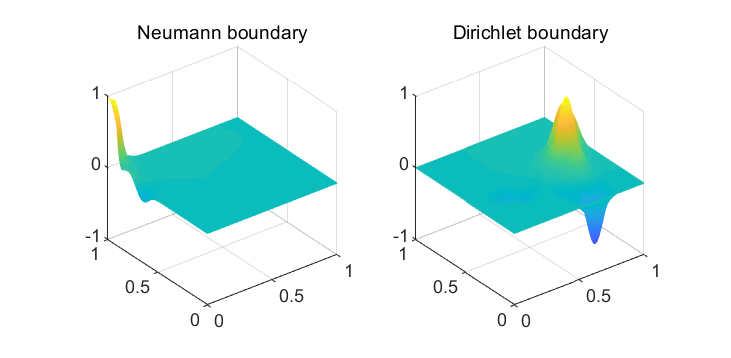
\includegraphics[width=0.45\linewidth]{pic/me2d3}
    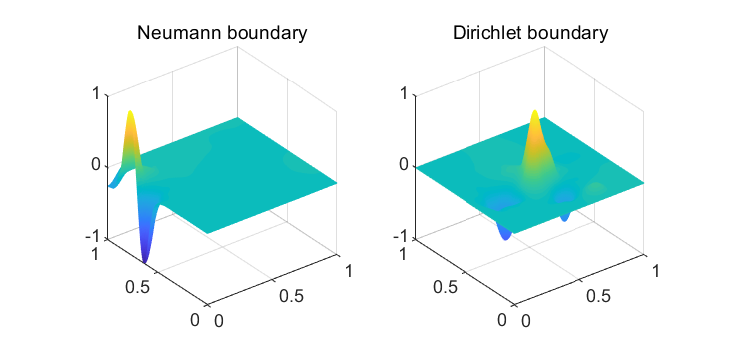
\includegraphics[width=0.45\linewidth]{pic/me2d5}
    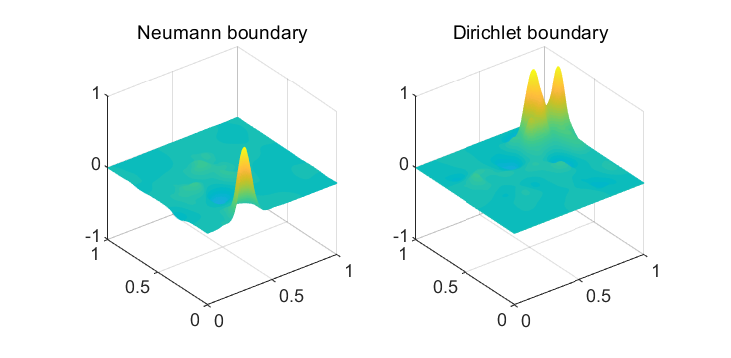
\includegraphics[width=0.45\linewidth]{pic/me2d20}
    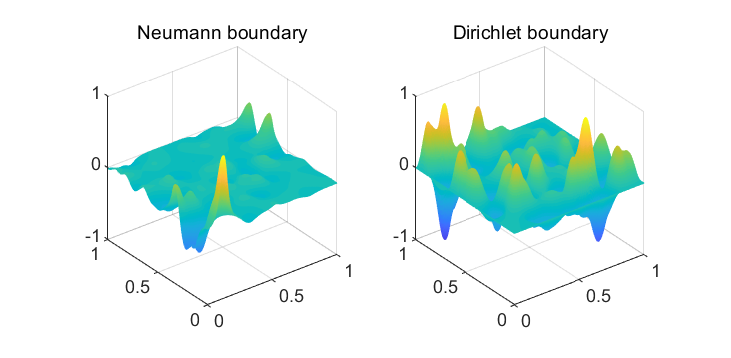
\includegraphics[width=0.45\linewidth]{pic/me2d50}
    \label{fig12}
\caption{不同边界条件下eignemode的比较(编号依次为1,2,3,5,20,50)}
\end{figure}

在这里,一维和二维的例子有很大的区别。在前面的两个例子中,我们同样取K为3000,势函数为$[0,K]$内的均匀分布。画出两种不同边界下的特征值如图\ref{fig13}。图中横轴为特征值编号(第几小的特征值),纵轴为特征值的数值。

\begin{figure}[htbp]
    \centering
    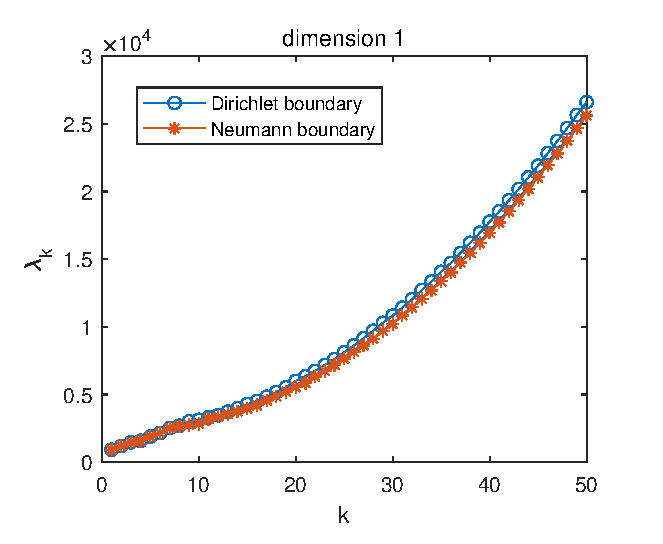
\includegraphics[width=0.45\linewidth]{pic/lam1d}
    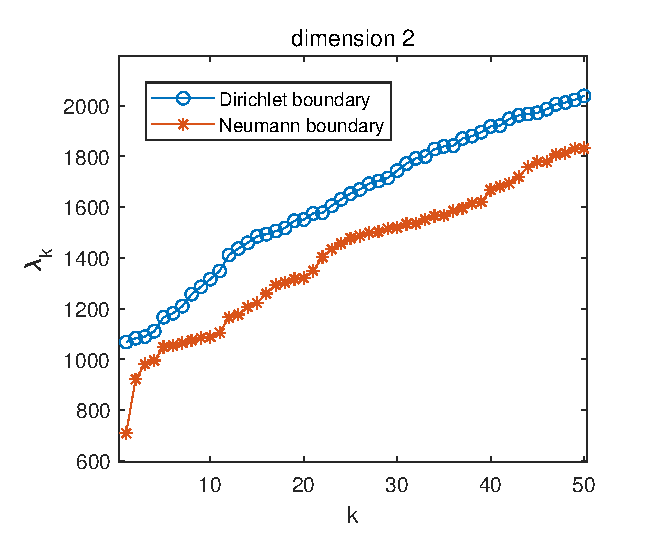
\includegraphics[width=0.45\linewidth]{pic/lam2d}
    \label{fig13}
\caption{不同边界条件下特征值的数值}
\end{figure}

可以看出,一维情况,两种边界条件下对应排序的特征值相差很小,但是二维的时候就相差很大。((这个也可以验证特征值增长的阶)

\section{画出valley line}

目前得valley line画出来是这样。两篇文章里都提到了watershed,这可能是个算法,具体还不清楚。
\begin{figure}[htbp]
    \centering
    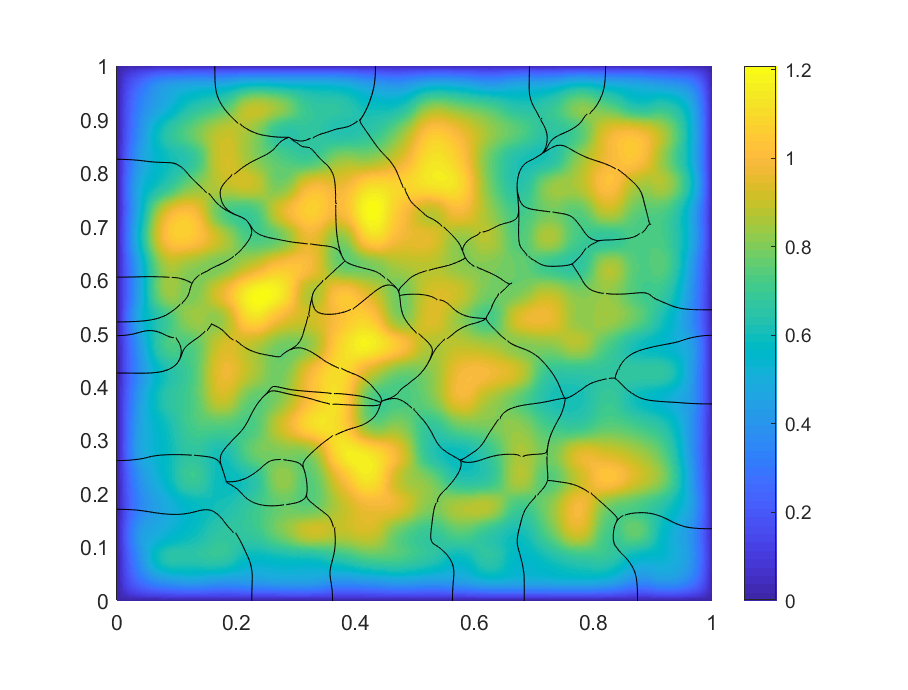
\includegraphics[width=0.4\linewidth]{pic/vline4}
    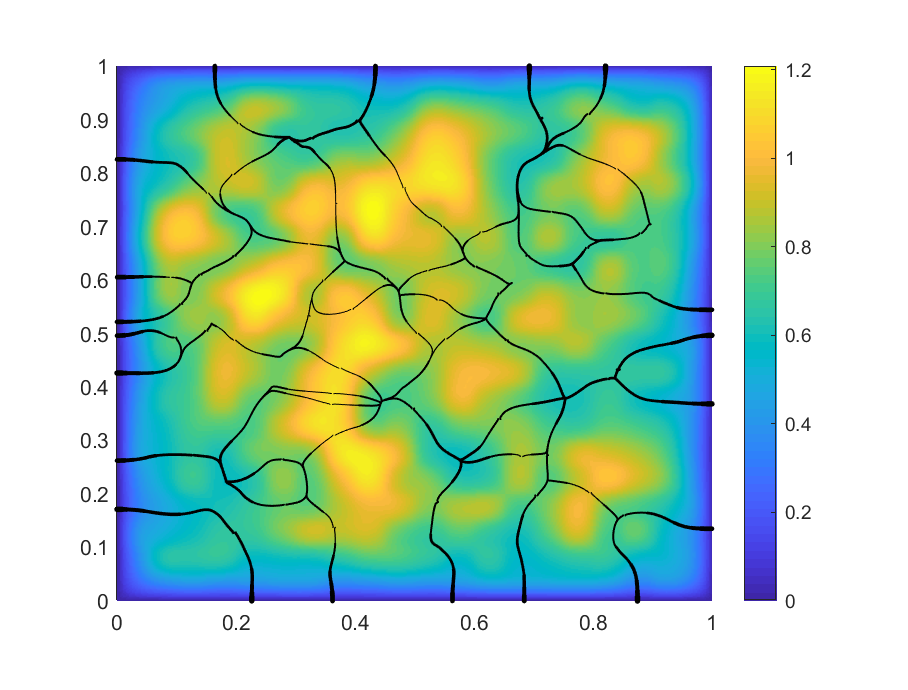
\includegraphics[width=0.4\linewidth]{pic/hvline4}
    \label{figv1}
\caption{K=3000,均匀分布}
\end{figure}




\end{document}